\chapter{Grundlegende Konzepte}

Die Software unterscheidet zwischen zwei Typen von Ausgaben:

\begin{itemize}[nosep]
	\item Regelmäßige Ausgaben
	\item Einzigartige Ausgaben
\end{itemize}

\section{Regelmäßige Ausgaben} \label{sec:fixedExpenses}

Regelmäßige bzw. wiederkehrende Ausgaben treten in einem bestimmten Rhythmus auf (bspw. vierteljährlich oder monatlich).

\begin{figure}[h!]
	\centering
	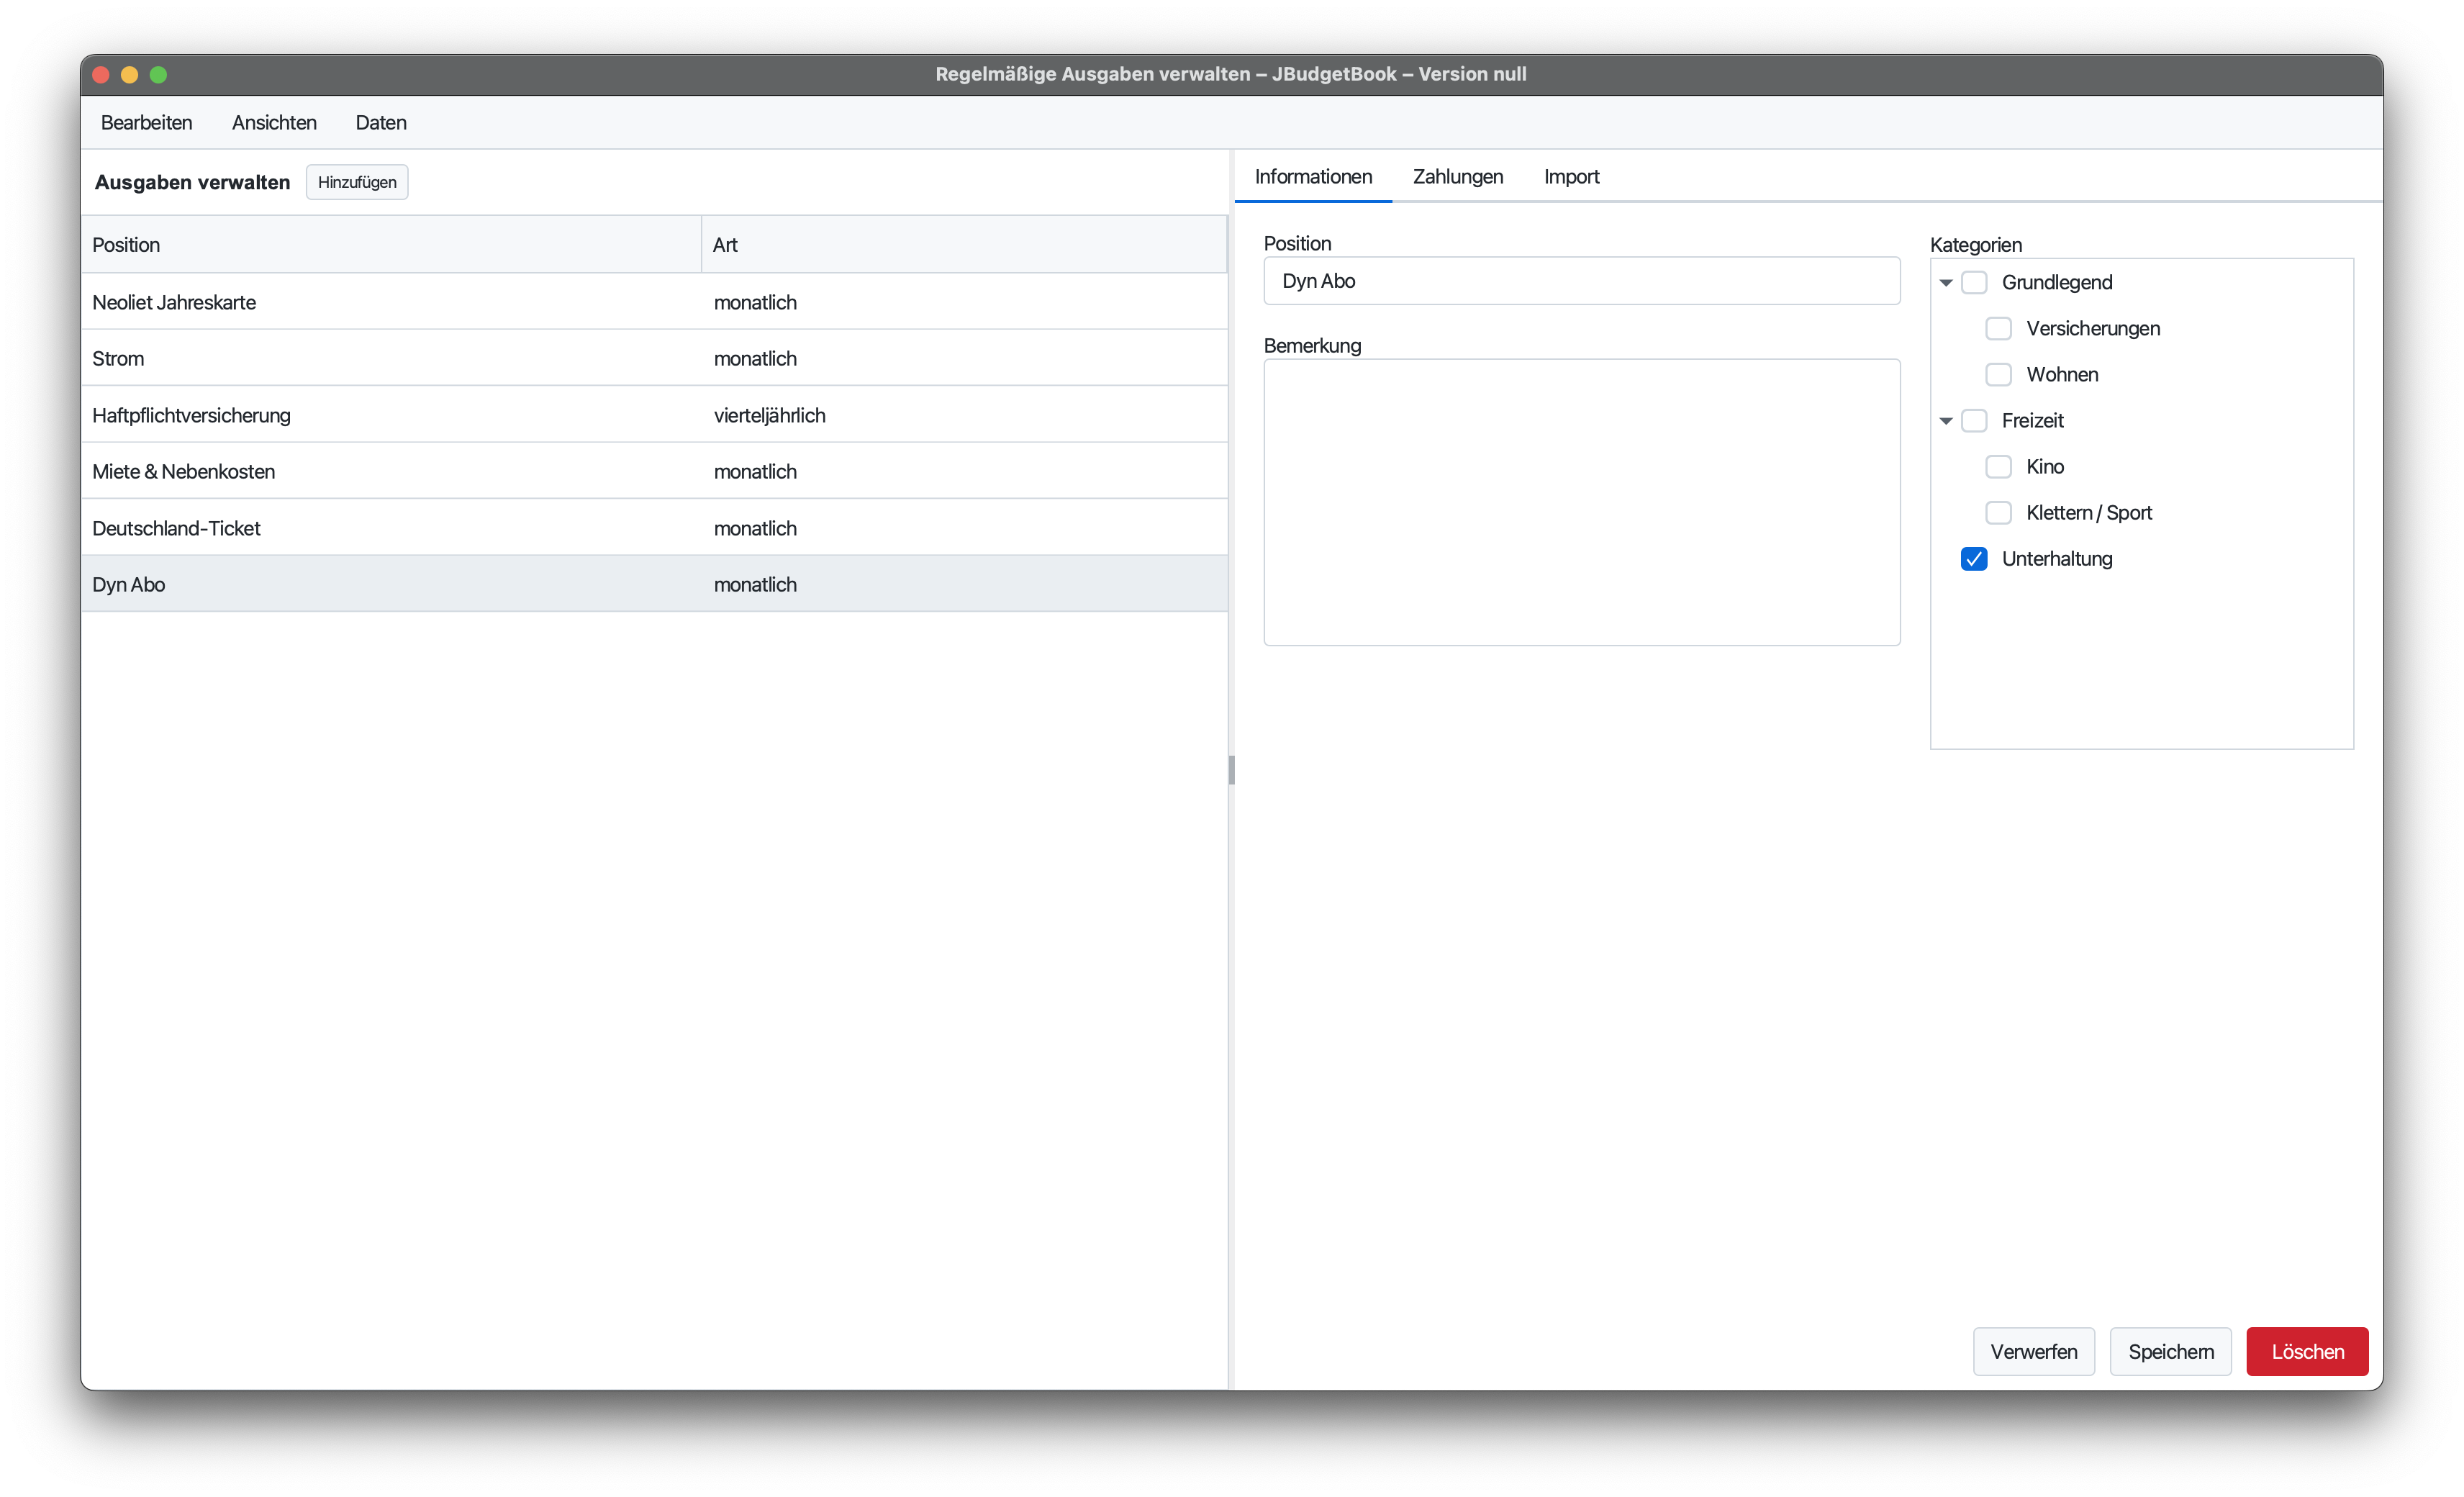
\includegraphics[width=\textwidth]{img/Screenshot-FixedExpenses-MDV}
	\vspace{-2em}
	\caption{Listen- \& Detailansicht der regelmäßigen Ausgaben}
	\label{fig:mdvFixedExpenses}
\end{figure}

In der Detailansicht (s. Abbildung \ref{fig:mdvFixedExpenses} rechts) kann u. a. der Zyklus/Rhythmus der Ausgabe und die Importregel festgelegt werden. 

\begin{infobox}
\textbf{Hinweis zu importieren Umsätzen}: Sollten zu einer Ausgabe reale Umsätze importiert worden sein, werden in den Übersichten (bspw. Monatsansicht) der Betrag dieser importierten Umsätze verwendet und der im System konfigurierte Betrag nur noch als Fallback verwendet. 
\end{infobox}

Da reale Ausgaben (bzw. Importe) über die Importregeln einer regelmäßigen Ausgabe zugeordnet werden können und dann dieser reale Umsatz in der Software angezeigt wird, können auch wiederkehrende Ausgaben mit schwankenden Beträgen -- wie es beim Tanken der Fall ist -- gruppiert werden.


\section{Einzigartige Ausgaben}

Einzigartige Ausgaben bzw. einmalige Ausgaben treten einmalig oder selten auf, sodass es keinen Mehrwert bietet, diese als regelmäßige Ausgaben zu gruppieren (da bspw. keine wiederkehrende Importe zu Ausgaben dieser Art erwartet werden.